\nonstopmode
\documentclass[10pt, a4paper]{article}
%\usepackage{subfig}

\parindent=20pt
\parskip=8pt
\usepackage[width=15.5cm, left=3cm, top=2.5cm, height= 24.5cm]{geometry}
\usepackage[english]{babel}
\usepackage[utf8]{inputenc}
\usepackage{fancyhdr}
\usepackage{multirow}
\usepackage{rotating}
\usepackage{tabto}
\usepackage{indentfirst}
\usepackage{latexsym}
\usepackage{gnuplottex}
\usepackage{epsfig}
\usepackage{lastpage}
\usepackage{amsfonts}
\usepackage{listings}
\usepackage[export]{adjustbox}
\usepackage{pdfpages}
\lstset{language=C}
\usepackage[ruled,vlined,linesnumbered]{algorithm2e}
\usepackage{graphicx}
\usepackage{float}
\usepackage{color}
\usepackage{amssymb}
\usepackage{caratula}
\graphicspath{{imgs/}}
\setlength{\parindent}{0pt}


% Acomodo fancyhdr.
\pagestyle{fancy}
\thispagestyle{fancy}
\addtolength{\headheight}{1pt}
\lhead{Algoritmos y Estructuras de Datos III}
\rhead{TP1}
\cfoot{\thepage /\pageref{LastPage}}
\renewcommand{\footrulewidth}{0.4pt}
\renewcommand{\thesubsubsection}{\thesubsection.\alph{subsubsection}}


\newenvironment{changemargin}[2]{%
\list{}{\rightmargin#2\leftmargin#1
\parsep=0pt\topsep=0pt\partopsep=0pt}
\item[]}
{\endlist}

\newenvironment{indentmore}{\begin{changemargin}{1cm}{0cm}}{\end{changemargin}}


\author{Algoritmos y Estructuras de Datos III, DC, UBA.}
\date{}
\title{}


\begin{document}

		
	\materia{Algoritmos y Estructuras de Datos III} % obligatorio
	\submateria{Segundo Cuatrimestre de 2015} % opcional
	\titulo{Trabajo practico 1} % obligatorio
	
	
	\integrante{Integrante Ignacio Rodriguez}{797/13}{igna\_nacho286@hotmail.com} % obligatorio 
	\integrante{Integrante Matias Visgarra}{567/11 }{matias\_kingthor@hotmail.com} % obligatorio 
	\integrante{Integrante Nicolás Mastropasqua}{828/13}{me.nicolas7@gmail.com} % obligatorio 
	\integrante{Integrante Fermín Travi}{234/13}{fermintravi@gmail.com} % obligatorio 
	
	
	\maketitle
	% compilar 2 veces para actualizar las referencias
	\tableofcontents
	
	\pagebreak
\section{Problema 1: Tel\'egrafo}
\subsection{Descripci\'on del problema}

El problema del tel\'egrafo consiste en conectar mediante un cable de tel\'egrafo a las estaciones de los ramales del sistema f\'erreo que se encuentra en el pa\'is, sabiendo que cada ramal dispone de una cierta cantidad de cable para conectar sus estaciones, cuya longitud se mide en kil\'ometros. \\
Lo que buscamos conseguir es que dado un ramal con sus estaciones y los kil\'ometros de cable de los que dispone, saber cual es el mayor n\'umero de estaciones seguidas que se pueden conectar con dicho cable. Para esto contamos con los ramales y sus estaciones, la distancia en kil\'ometros de cada una de las estaciones  a la capital, que se encuentra en el kil\'ometro $0$, y la cantidad de cable de la que dispone cada ramal.\\
En los datos de entrada, cada ramal ocupa dos lineas. La primera representa los kil\'ometros de cable de los que dispone dicho ramal, y la segunda las distancias de las estaciones del ramal a la capital.\\
Como datos de salida, el algoritmo encargado de resolver el problema debe devolver una linea por cada ramal, donde cada linea indica la cantidad m\'axima de estaciones de dicho ramal que se pueden conectar con el cable de tel\'egrafo.
\begin{flushleft}
\textbf{Ejemplos:}\\
\end{flushleft}

\begin{enumerate}
	\item \textbf{Kil\'ometros de cable:} 6. \textbf{Distancia de las estaciones:} 6 8 12 15.\\
	En este ejemplo la m\'axima cantidad de estaciones que puedo conectar con 6 kil\'ometros de cable es 3, las cuales son las que se encuentran en el kil\'ometro 6, 8 y 12, ya que desde las estaciones que se encuentran en el kil\'ometro 0 y el 8 solo puedo conectar 2, las que se encuentran en el kil\'ometro 0 y 6 para la primera, y las que se encuentran en el kil\'ometro 8 y 12 para la segunda.
	\item \textbf{Kil\'ometros de cable:} 6. \textbf{Distancia de las estaciones:} 7 14 21 28.\\
	En este caso, la distancia entre cada una de las estaciones es mayor que la cantidad de kil\'ometros de cable del que se dispone, por lo que la soluci\'on de este caso es que hay 0 estaciones que se pueden conectar mediante el cable.
	\item \textbf{Kil\'ometros de cable:} 6. \textbf{Distancia de las estaciones:} 3 6 9 12 15 18.\\
	En este \'ultimo caso las distancias entre todas las estaciones es la misma, y con los kil\'ometros de cable de los que disponemos podemos conectar como m\'aximo hasta 3 estaciones.
	
\end{enumerate}
\subsection{Resoluci\'on}
Lo que nuestro algoritmo hace primero es buscar, en un vector con las distancias de las estaciones del ramal a la capital llamado $distanciaDeLasEstaciones$, la m\'axima cantidad de estaciones que puedo conectar con la capital, lo cual me va a servir como cota m\'inima de la cantidad m\'axima de estaciones que puedo conectar. \\Para esto recorro el vector linealmente hasta encontrar la \'ultima estaci\'on alcanzable desde la capital con el cable. El valor resultante lo guardo en $maximaCantidadDeEstaciones$, que va a servir para almacenar la m\'axima cantidad de estaciones conectables con el cable de tel\'egrafo.\\
Luego, utilizando dos \'indices, $inicio$ y $fin$, vuelvo a recorrer $distanciaDeLasEstaciones$ para encontrar la m\'axima cantidad de estaciones que voy a poder conectar con el cable. Los \'indices $inicio$ y $fin$ van a representar la posici\'on de las estaciones dentro del vector $distanciaDeLasEstaciones$, y van a comenzar inicializados con valores 0 y 1 respectivamente. \\La manera en la que voy ir recorriendo dicho vector es ir aumentando el valor de $fin$ hasta que la cantidad de estaciones entre $inicio$ y $fin$ supere el valor de $maximaCantidadDeEstaciones$ o me quede sin estaciones para recorrer.\\
En caso de que suceda lo primero reemplazo el contenido de $maximaCantidadDeEstaciones$ por la cantidad de estaciones entre $inicio$ y $fin$(sin contar la \'ultima estaci\'on a la que el cable no llega), aumento en uno el valor de $inicio$, y vuelvo a comenzar a aumentar el valor de $fin$.\\ 
Por otro lado, como $inicio$ no puede ser mayor que $fin$, si cuando tengo que aumentar el valor de $inicio$ este iguala al valor de $fin$, en ves de aumentar \'unicamente $inicio$, aumento el valor de ambos \'indices en uno.\\
Cuando me quede sin estaciones para recorrer devuelvo el valor de $maximaCantidadDeEstaciones$ como resultado del problema.\\
\begin{flushleft}
Para finalizar, a continuaci\'on mostramos un pseudoc\'odigo de lo explicado anteriormente.
\end{flushleft}


\begin{algorithm}[H]
	\SetAlgoLined
	\caption{Tel\'egrafo}
	\KwIn{int $kilometrosDeCable$, vector$<$ int$>$ $distanciaDeLasEstaciones$}
	int $inicio$ $\leftarrow$ 0\\
	int $fin$ $\leftarrow$ 1\\
	int $cantidadDeEstaciones$ $\leftarrow$ 0\\
	int $maximaCantidadDeEstaciones$ $\leftarrow$ \'ultima estaci\'on alcanzable desde la capital con el cable\\
	mientras $fin$ $<$ total de estaciones del ramal\\
	 $\ \ \ \ \ \ $ Si puedo unir con cable las estaciones entre $inicio$ y $fin$\\
	 $\ \ \ \ \ \ \ \ \ \ \ \ $ $ cantidadDeEstaciones$ $\leftarrow$ La cantidad de estaciones entre $inicio$ y $fin$ \\
	 $\ \ \ \ \ \ \ \ \ \ \ \ $ Si $cantidadDeEstaciones$ $>$ $maximaCantidadDeEstaciones$\\
	 $\ \ \ \ \ \ \ \ \ \ \ \ \ \ \ \ \ \ $ $maximaCantidadDeEstaciones$ $\leftarrow$ $cantidadDeEstaciones$\\
	 $\ \ \ \ \ \ \ \ \ \ \ \ $ Aumento el valor de $fin$ en 1\\
	 $\ \ \ \ \ \ $ Si no puedo unir las estaciones entre $inicio$ y $fin$ con el cable\\
	 $\ \ \ \ \ \ \ \ \ \ \ \ $ Si $fin$ es igual a $inicio$+1 aumento ambos \'indices en 1\\
	 $\ \ \ \ \ \ \ \ \ \ \ \ $ Si no, aumento \'unicamente $inicio$ en 1\\
	 Devuelvo el valor almacenado en $maximaCantidadDeEstaciones$
\end{algorithm}

\subsection{Justificaci\'on}
Como se menciona en el algoritmo explicado en el punto anterior, se van a recorrer las estaciones del ramal, las cuales se encuentran en el vector $distanciaDeLasEstaciones$, utilizando los \'indices $inicio$ y $fin$. \\
Se va a ir aumentando el valor del \'indice $fin$ mientras pueda seguir conectando las estaciones con el cable, y cuando no pueda conectarlas se va a ir aumentando el \'indice $inicio$ hasta poder volver a hacerlo. Eso quiere decir que por cada valor que toma el \'indice $inicio$ se va a buscar la \'ultima estaci\'on que se pueda conectar con el cable a partir de dicho \'indice, actualizando el valor de $maximaCantidadDeEstaciones$ si la cantidad de estaciones supera su valor. \\
Por ende, como el valor de $maximaCantidadDeEstaciones$ solo almacena la m\'axima cantidad de estaciones conectables por el cable de tel\'egrafo, y desde cada estaci\'on marcada con el \'indice $inicio$ calculo la m\'axima cantidad de estaciones que puedo conectar con el cable desde dicha estaci\'on, $maximaCantidadDeEstaciones$ va a terminar almacenando el valor de la m\'axima cantidad de estaciones desde alguna estaci\'on, es decir, la respuesta al problema.

\subsection{Complejidad}

Llamemos $n$ a la cantidad de estaciones. Como lo que hace el algoritmo es recorrer con dos \'indices el vector de estaciones de tama\~no $n$, y ninguno de los dos \'indices decrece, al final lo que termina haciendo es recorrer el vector de estaciones hasta el final con cada \'indice. La complejidad de recorrer un vector dos veces es $O(2n)$, que es lo mismo que $O(n)$.\\
Por otro lado, a parte de recorrer el vector de estaciones, lo que hace el algoritmo es hacer acceder a dicho vector mientras lo recorre y hacer cuentas entre las estaciones ubicadas en los \'indices $inicio$ y $fin$ del vector para saber si se pueden conectar mediante el cable de tel\'egrafo, actualizar el valor de $maximaCantidadDeEstaciones$, y aumentar el valor de los \'indices, todo lo cual tiene una complejidad $O(1)$.\\
Por todo lo anterior, la complejidad final del algoritmo es $O(n)$.

\subsection{Casos de Test}

Para corroborar el correcto funcionamiento del algoritmo, este mismo de probo con el siguiente conjunto de tests.

\begin{enumerate}
	\item \textbf{Kil\'ometros de cable:} 5. \textbf{Distancia de las estaciones:} 6 12 18 24\\
	Este primer test se utiliz\'o para corroborar que el algoritmo devolviera 0 en caso de que no se pudiera conectar ninguna estación mediante el cable, dado que la distancia entre cada una de las estaciones es mayor que la cantidad de kil\'ometros de cable disponible.
	
	\item \textbf{Kil\'ometros de cable:} 0. \textbf{Distancia de las estaciones:} 3 8 12 17\\
	Este test se utiliz\'o para corroborar que si la cantidad de cable disponible para conectar las estaciones es 0, el algoritmo devolviera 0, ya que sin cable las estaciones no se pueden conectar.
	
	\item \textbf{Kil\'ometros de cable:} 6. \textbf{Distancia de las estaciones:} 6 8 12 15\\
	Este test, dado por la c\'atedra, se utiliz\'o para corroborar el correcto funcionamiento del algoritmo dado una instancia normal, es decir, una instancia sin ning\'un caso especial.
	
	\item \textbf{Kil\'ometros de cable:} 34. \textbf{Distancia de las estaciones:} 6 10 22 34\\
	Este test sirvi\'o para corroborar que si el cable alcanzara para conectar todas las estaciones, el algoritmo devolviera la cantidad total de estaciones, incluida la de la capital, como resultado. 
	
	\item \textbf{Kil\'ometros de cable:} 5. \textbf{Distancia de las estaciones:} 5 10 15 20 25\\
	Por \'ultimo, este test se utiliz\'o para corroborar que si la distancia entre todas las estaciones fuera igual a la cantidad de cable, el algoritmo devolviera 2 como resultado, ya que solo dos estaciones se pueden conectarse mediante el cable.
\end{enumerate}

\subsection{Tiempos de ejecuci\'on y gr\'aficos}

Para poder observar la performance en t\'erminos de tiempo del problema, se corrieron los siguientes casos de tests, variando en cada uno la cantidad de estaciones del ramal, la cantidad de cable de tel\'egrafo disponible para conectar las estaciones, y la distancia entre dichas estaciones.

\begin{enumerate}
	\item En el primer test utilizado para observar el tiempo de ejecuci\'on del problema, la cantidad de cable que se utiliz\'o para poder conectar las estaciones fue de 200.\\ El mismo test se corri\'o 1000 veces, en donde en cada iteraci\'on la cantidad total de estaciones iba aumentando en 100, es decir, comienza con 100 estaciones en la primera iteraci\'on del test, y para la \'ultima iteraci\'on termina con 100000 estaciones. Luego, para cada una de las iteraciones del test, la distancia entre cada una de las estaciones se mantuvo en 10.\\
	El figura 1 muestra el resultado de dicho test.\\
	\begin{figure}[H]
  		\centering
   	 	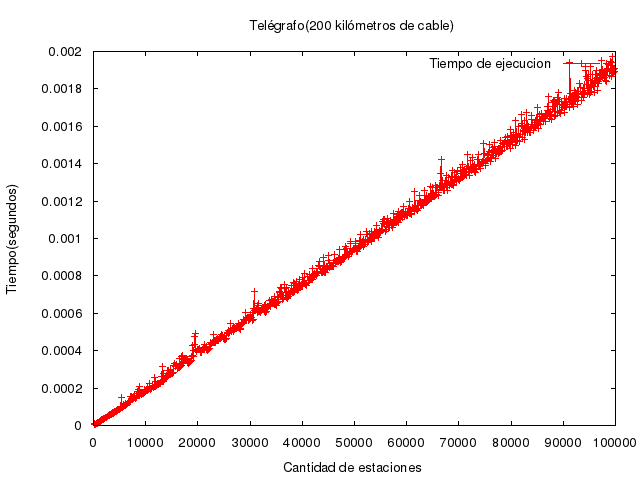
\includegraphics[width=1\textwidth]
   	 	{Imagenes/telegrafoTiempos1.png}
		\caption{Primer test}
	\end{figure}
	
	\item Para el segundo test se mantuvieron los mismos datos que para el primero, a excepci\'on de la cantidad de cable, que se disminuyo a 50.\\ Como puede verse en la figura 2, el tiempo que tardo en resolver el mismo problema pero con una cantidad de cable menor es el mismo, con lo que podemos afirmar que la cantidad de cable utilizada para conectar las estaciones no influye en el tiempo, teniendo en cuenta que la distancia entre estaciones es menor que la cantidad de cable disponible.\\
	\begin{figure}[H]
  		\centering
   	 	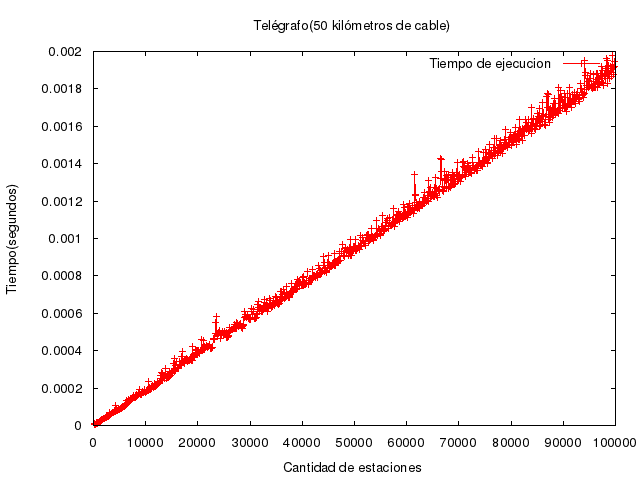
\includegraphics[width=1\textwidth]
   	 	{Imagenes/telegrafoTiempos2.png}
		\caption{Segundo test}
	\end{figure}
	
	\item Ahora, en el tercer test, para poder observar si la distancia entre las estaciones influye en el tiempo de ejecuci\'on del problema, se corrieron las mismas instancias que en el primer test, salvo que ahora la distancia entre cada una de las estaciones se hizo de 220, de manera que la cantidad de cable no alcanzara para conectar ninguna estaci\'on.\\
	En la figura 3 puede observarse que el tiempo de ejecuci\'on de dicha instancia decreció respecto de lo que tardo en el primer test. Esto sucede porque cada vez que el algoritmo no puede conectar una estaci\'on con la siguiente mediante el cable pasa a la siguiente estaci\'on para corroborar lo mismo. Esto resulta en que el arreglo de estaciones se recorra una \'unica vez, en vez de un total de 2 veces si siempre encuentra una estaci\'on para poder conectar mediante el cable.\\
	\begin{figure}[H]
  		\centering
   	 	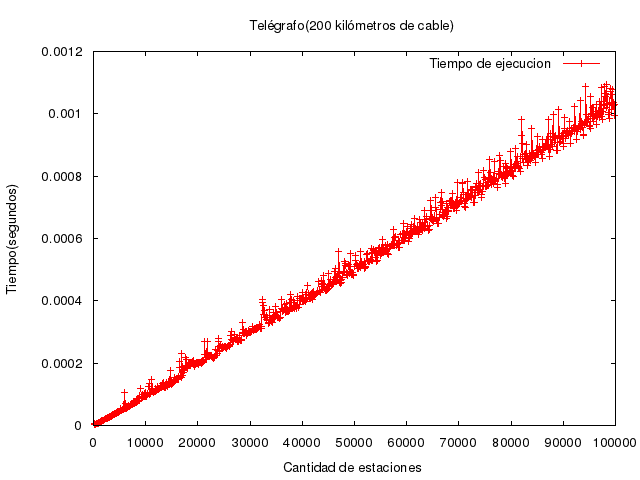
\includegraphics[width=1\textwidth]
   	 	{Imagenes/telegrafoTiempos6.png}
		\caption{Tercer test}
	\end{figure}
	
	\item El siguiente test se utiliz\'o para corroborar si la cantidad de estaciones efectivamente influye en el tiempo de ejecuci\'on. En este caso, se tomaron los mismos valores que en el primer test, pero se aumento la cantidad de iteraciones del test a 30000, es decir, que para la \'ultima iteraci\'on del test la cantidad de estaciones se hace de 300000.\\ 
	En la figura 4 se aprecia claramente que, como era de esperarse, mientras mas estaciones haya que revisar, mas tiempo le toma al algoritmo encontrar la soluci\'on al problema.\\
	\begin{figure}[H]
  		\centering
   	 	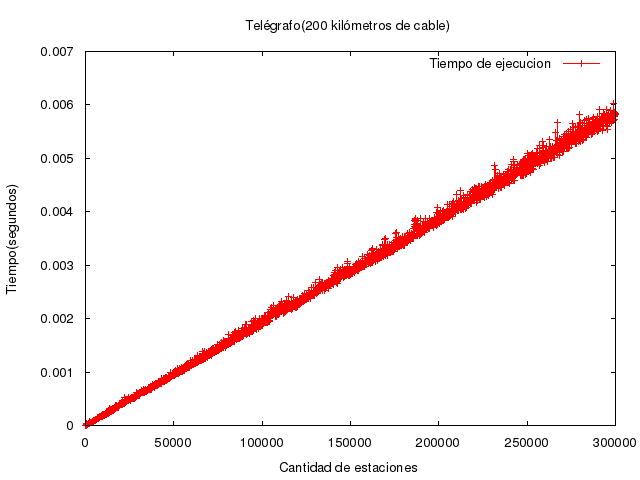
\includegraphics[width=1\textwidth]
   	 	{Imagenes/telegrafoTiempos3.png}
		\caption{Cuarto test}
	\end{figure}
	
	\item Para terminar, el siguiente test fue utilizado para corroborar que la complejidad del algoritmo fuera la esperada. Para eso, se corrieron la misa cantidad de instancias que para el test 1 y con los mismos par\'ametros a excepci\'on de la distancia entre cada una de las estaciones. En este caso cada estaci\'on esta separada aleatoriamente entre 100 y 200 kil\'ometros de la siguiente estaci\'on.\\
	Luego, a los tiempos resultantes de dicha experimentaci\'on se los dividió por el tama\~no de la entrada, es decir, la cantidad de estaciones en cada iteraci\'on del test. \\
	Las figuras 5 y 6 muestran el tiempo de ejecuci\'on de correr dicho test, y el resultado de dividir los tiempos obtenidos por el tama\~no de la entrada, y como puede observarse en la figura 6, la funci\'on de tiempo sobre tama\~no de entrada tiende a una constante, por lo que podemos asumir que la complejidad del algoritmo es, seg\'un lo esperado, $O(n)$.\\
	\begin{figure}[H]
  		\centering
   	 	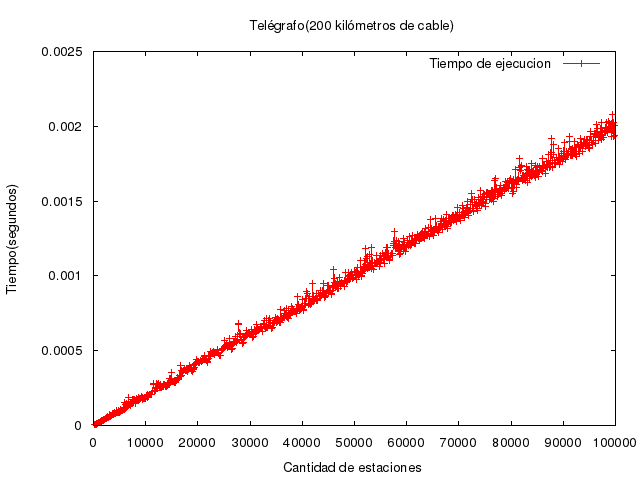
\includegraphics[width=1\textwidth]
   	 	{Imagenes/telegrafoTiempos4.png}
		\caption{Quinto test}
	\end{figure}
	
	\begin{figure}[H]
  		\centering
   	 	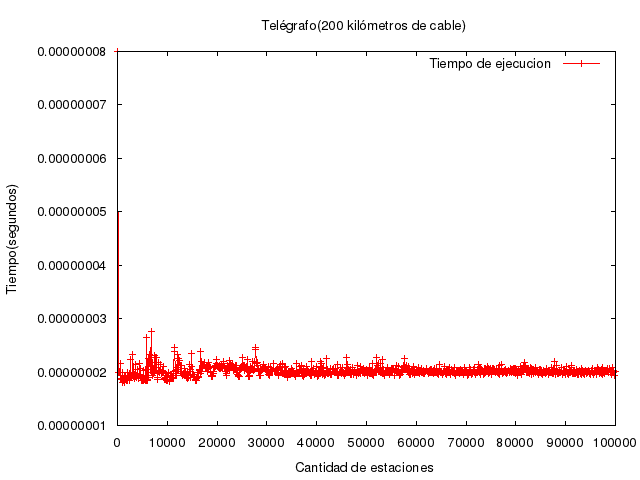
\includegraphics[width=1\textwidth]
   	 	{Imagenes/telegrafoTiempos4Comparando.png}
		\caption{Quinto test comparando con tama\~no de la entrada}
	\end{figure}
	\end{enumerate}
\section{Problema 2: A Medias}
		\subsection{Descripci\'on del problema:}
		El problema que se nos present\'o consist\'ia en, mediante un arreglo ya formado, crear uno nuevo que en la posici\'on $i$ de este nuevo arreglo tuviese la mediana del subarreglo ordenado que se forma del arreglo original entre las posiciones 0 a $i$.
		\\ La mediana para un arreglo de tama\~no \textit{n}  se calcula de la siguiente forma: si el arreglo tiene un tama\~no impar la mediana es \textit{x$_{(n+1)/2}$}; en cambio, si el tama\~no es par, es (\textit{x$_{(n)/2}$}+\textit{x$_{(n+1)/2}$})$/2$.
		\subsection{Resoluci\'on del problema:}
		Para resolver el problema se decidi\'o usar una estructura que consiste de cuatro observadores: dos heaps (un min heap y un max heap), un entero que contiene a la mediana y un entero que representa el tamaño del arreglo.
		\\ Para armar el arreglo que se va a devolver, se recorre el arreglo original, se toma el valor que est\'a en la posici\'on $i$ del arreglo original y luego se analiza el tama\~no del subarreglo (antes de agregar un nuevo n\'umero). En caso de que sea 0, quiere decir que esta vac\'io, entonces la mediana es el valor que tomamos.
		\\Si el subarreglo tiene un tama\~no impar, nos fijamos si el valor es mayor o menor que la mediana. En caso de que sea menor, se agrega el valor al max heap y la mediana al min heap, y si es mayor es al rev\'es. Luego, la mediana es la suma de las ra\'ices de los heaps dividido dos y se le suma 1 al tama\~no.
		\\En cambio, si el subarreglo tiene tama\~no par, tambi\'en nos fijamos si el valor es mayor o menor que la mediana. En caso de ser menor, se le agrega el valor al max heap y se desencola la ra\'iz del max heap y ese se transforma en la mediana, pero si es mayor se agrega el valor al min heap y se desencola la ra\'iz del min heap y ese se transforma en la mediana, y se le suma uno al tama\~no.
		\\Como dijimos, esto se va a hacer mientras se recorre el arreglo original, entonces cada vez que se agrega un nuevo valor a la estructura nos fijamos cual es la mediana y agregamos la mediana al arreglo que vamos a devolver.
		\subsection{Justificación del algoritmo:}
		 La idea del algoritmo es que el tama\~no de los heaps siempre sea igual y de esa forma poder siempre ver f\'acilmente la parte que nos importa del subarreglo r\'apidamente y de una forma ordenada. Como ya se explic\'o anteriormente, antes de agregar un nuevo valor al subarreglo nos fijamos el tama\~no de este. Como caso base si el subarreglo tiene tama\~no 0 antes de agregar un n\'umero, cuando lo agreguemos va a tener tama\~no 1 y en ese caso ese mismo n\'umero va a ser la mediana, y los dos heaps tienen tama\~no cero.
		\\Ahora suponiendo que ambos heaps tienen el mismo tama\~no:
		\\ En caso de que antes de agregar un n\'umero el tama\~no sea impar, cuando lo agreguemos va a ser par, entonces por la f\'ormula para calcular la mediana tenemos que sumar los dos n\'umeros que est\'an en el medio y dividirlos por dos, pero antes de hacer eso hay que fijarse si el valor que se va a agregar es mayor o menor que la mediana y a qu\'e heap tendr\'ia que ir.
		\\Si el valor es menor que la mediana, se agrega el valor al max heap, que es donde est\'an los valores menores que la mediana, y la mediana se agrega al min heap, que es donde est\'an los valores mayores que la mediana, y de esta forma se mantiene el invariante de que los dos heaps tienen el mismo tamaño, y le mediana nueva se calcula con la f\'ormula previamente mencionada.
		\\ Si en cambio el tama\~no es par, cuando lo agreguemos va a ser impar, entonces la mediana va a ser el elemento que est\'a en el medio. Ahora nos fijamos si el valor a agregar es mayor o menor que la mediana, en caso de ser menor lo agregamos al max heap y desencolamos su ra\'iz, y esa va a ser la nueva mediana. En caso de ser mayor se agrega al min heap y luego se desencola la ra\'iz. La ra\'iz desencolada va a ser la nueva mediana, y los tama\~no de los heap se mantienen equivalentes.
		\subsection{Complejidad del algoritmo:}
		La complejidad de este algoritmo es de \textit{nlog(n / 2)}, que asint\'oticamente es equivalente a \textit{O(nlogn)}, que es mejor que la cota que nos ped\'ian de \textit{n$^{2}$}, siendo \textit{n} la cantidad de n\'umeros que tiene el arreglo original. Esta complejidad se debe a que en cada iteraci\'on se realiza uno o dos adiciones a un heap, dependiendo esto del tama\~no del subarreglo, y se ven las ra\'ices de los heaps, pero al ser de tiempo constante esta funci\'on no suma a la complejidad, haciendo que cada adici\'on al subarreglo sea \textit{log(n)}. Como esto se realiza para todos los n\'umeros en el arreglo original, esto se realiza \textit{n} veces, haciendo que la complejidad total sea la dicha.
		\\Se sabe que los m\'etodos de des/encolar son de \textit{O(log n)} y ver la ra\'iz de \textit{O(1)} por la documentaci\'on de Java:
		\\Implementation note: this implementation provides O(log(n)) time for the enqueing and dequeing methods (offer, poll, remove() and add); linear time for the remove(Object) and contains(Object) methods; and constant time for the retrieval methods (peek, element, and size).
		\\A su vez, el tiempo promedio de agregar un elemento al heap es de \textit{O(1)}.
	\subsection{Tiempos de ejecuci\'on y gr\'afico}
	Para poder apreciar c\'omo var\'ian los tiempos dependiendo del tamaño del input, se realiz\'o el siguiente gr\'afico que incluye la ejecuci\'on del algoritmo con arreglos de distinto tama\~no. Para los casos de prueba se utilizaron n\'umeros pseudoaleatorios en el arreglo, generados mediante la librer\'ia $util.Random$ de Java. Como se puede observar en el gr\'afico, se cumple la complejidad de caso promedio para la adici\'on de elementos al heap (que es de $O(1)$), por lo que se obtiene una funci\'on casi lineal. 
	El tama\~no del input se fue incrementando inicialmente por 50 (de 50 a 1000), luego por 100 (de 1000 a 4000) y finalmente por 500 (de 4000 a 17000).
	\begin{figure}
  		\centering
   	 	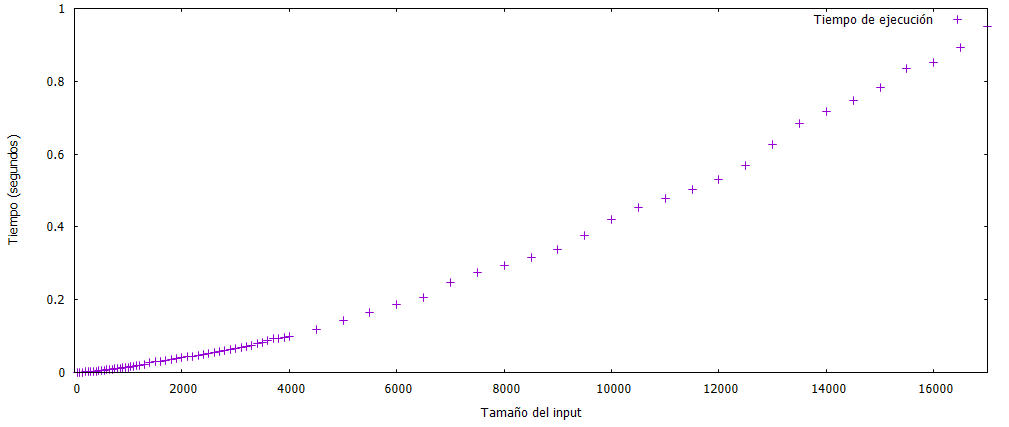
\includegraphics[width=1\textwidth]
   	 	{Imagenes/medianaTiempos.png}
		\caption{Tiempos variando el tama\~no del input}
	\end{figure}
	\\
	\newline
	\\Para el peor caso, se supuso que Java representa internamente al heap con un \'arbol binario, por lo que se dispuso a dise\~nar arreglos que fuercen a producir \textit{log n} intercambios cada vez que se realizaba una adici\'on al heap.
	\\Los arreglos que cumpl\'ian con esa propiedad eran aquellos que contenían n\'umeros en orden creciente en sus posiciones pares y n\'umeros en orden decreciente en sus posiciones impares (por ejemplo, (3, 89, 7, 62, 13, 50, 19, 43). De esta manera, por c\'omo se encuentra armado el algoritmo, siempre se agregaban elementos mayores que la ra\'iz al max heap y siempre se agregaban elementos menores que la ra\'iz al min heap (por lo que, te\'oricamente, se realizaban \textit{log n} intercambios en cada encolamiento).
	\\Sin embargo, al realizar los tests, si bien en un principio los tiempos eran mayores, al aumentar el tama\~no  del input, la funci\'on crec\'ia linealmente. Al desconocer c\'omo representa Java internamente a las colas de prioridad, no pudimos formar un caso que sea el peor.
	\\El tama\~no del input se fue aumentando en 100 desde el 0 al 1000 y en 500 del 1000 al 5000.
	\begin{figure}
  		\centering
   	 	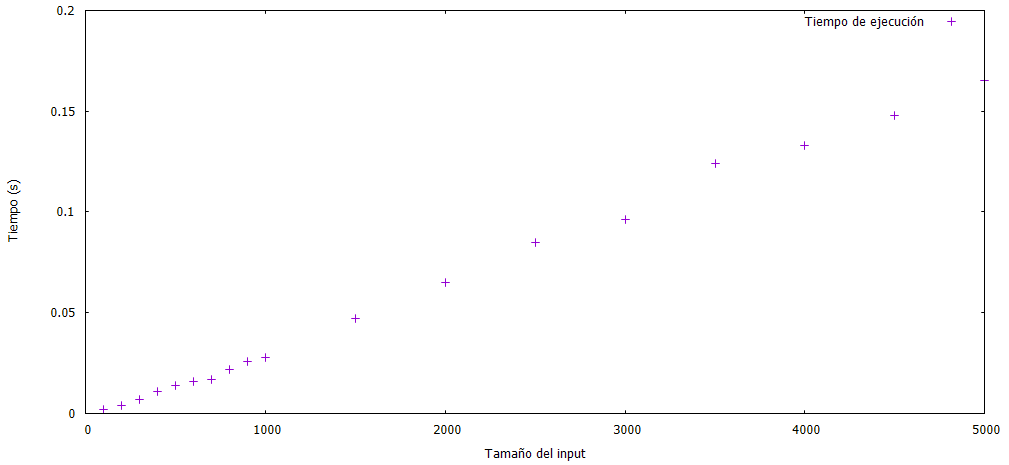
\includegraphics[width=1\textwidth]
   	 	{Imagenes/medianaPeorTiempos.png}
		\caption{Tiempos del peor caso variando el tama\~no del input}
	\end{figure}

\section{Problema 3: Girl Scouts}
\subsection{Descripción del problema:}


El problema consiste en obtener a partir de una lista de exploradoras, con forma de ronda y un peso entre cada par de elementos determinado por la distancia entre estos, 
obtener una permutación de ella tal que se haya minimizado la suma de los pesos de todos los elementos. Se debe devolver dicha lista en el orden que cumpla con 
la condición y un numero correspondiente a el peso máximo entre dos elementos de la ronda obtenida. En caso de existir mas de una solución, se debe devolver la de menor
orden lexicográfico.Notar que si dos elementos no están relacionados, no son amigas, entonces el peso es nulo.

\begin{flushleft}
\textbf{Ejemplos:}\\
\end{flushleft}
\begin{enumerate}

\item

Se tiene la siguiente lista, vista como una ronda:
$l =  [a, b, c, d]$ y la siguiente relación de amistad $a = {(a,c)(c,d)}$
La solución debe ser: $l' = [a, b, d, c]$ ya que $d(a,c)$  y $d(d,c)$ son uno, que es lo mínimo que se puede conseguir. Es importante ver que la distancia
,al ser una ronda, es siempre el $MIN{posicion(y) - posicion(x),longitudRonda - posicion(y) +posicion(x)}$ con $x$ e $y$  dos elementos cualesquiera .
Luego, esta solución es la mas chica ordenada de forma lexicográfica.
Notar que, entonces, la suma de las distancias totales, que fue minimizada, es : d(a,c)+d(d,c)+0 = 2.
Finalmente, el output debe ser: $1 [a, b, d, c]$ pues 1 es la distancia máxima entre cualquier par de elementos.

\item
Se tiene la siguiente lista, vista como una ronda:
$l = [a, b, c]$ y la siguiente relación de amistad $a = {(a,c)}$
La solución debe ser: $l' = [a,b,c]$ ya que $d(a,c) = 1$. A
Finalmente, el output debe ser:$ 1 [a, b, c]$ pues 1 es la distancia máxima entre cualquier par de elementos y la lista es la menor de todas las que cumplen.

\item
Se tiene la siguiente lista, vista como una ronda:
$l = [a,b,c,d,e]$ y la siguiente relación de amistad $a = {(a,b)(a,c)(a,d)(a,e)(c,e)}$.
La solución debe ser: $l' = 2 [a,b,c,e,d]$. Notemos que si bien la lista $[a,b,d,c,e]$ cumple con ser una minimización, la misma es mayor lexicográficamente que $l'$. Podemos ver fácilmente que como a esta relacionada con todas, no importa el orden en el que se pongan, la suma de las distancias no cambia. Sin embargo, al pedir que $(c,e)$ también sean amigas, obliga a tener que elegir un orden apropiado para estas dos ultimas letras. Básicamente, deben ir "pegadas". Luego, el mejor lugar para ponerlas es aquella que acerque la "e" hacia la "c", para obtener la menor de las posibles soluciones.

\end{enumerate}
\subsection{Resolución:} 

\begin{flushleft}
\textbf{Estructura:}\\
\end{flushleft}

Para resolver el problema, se decidió dividirlo en un conjunto de módulos,clases, para poder abstraer mejor los detalles que no fuesen inherentes al problema principal en si, el de la minimización de las distancias.
En este sentido, se implementaron tres clases: Amistad,Ronda y Fogón. Este es el orden de abstracción, es decir la ultima mencionada utiliza los servicios de las de abajo, y así sucesivamente. A saber, la clase Ronda es solo una extensión de la clase ArrayList. La clase Fogón tiene dos miembros: RondaOptima y un Conjunto de amistades(HashSet$<$Amistad$>$).

	
\begin{flushleft}
\textbf{Ideas centrales:}\\
\end{flushleft}

Básicamente, implementaremos un algoritmo que haga backtracking sobre las posibles formas de ordenar una ronda de exploradoras y nos quedaremos con aquella que minimice la suma de las distancias. Esta misma sera la que quedara referenciada por el campo rondaOptima de la clase.
Para esto, cuando el algoritmo de backtracking encuentre una primera permutación de la ronda, esta sera nuestra candidata a óptima. Luego,el algoritmo ira explorando nuevas soluciones posibles. Cuando llegue a una hoja del árbol de posibilidades, es decir, cuando quede definida una ronda que es permutación de la original se preguntara si la nueva suma de distancias es mejor. Si es así, habremos obtenido una nueva rondaOptima. De esta forma continuaremos hasta haber inspeccionado todas las posibles soluciones que sean relevantes(que podrían no ser todas, por las posibles podas).

Mas en detalle, diremos que la clase fogón cuenta con dos funciones: \textbf{Solve} y \textbf{SentarExploradoras}, que hace el trabajo mencionado arriba.
La primera recibirá una \textit{lista(ArrayList)} de exploradoras(Character) y un conjunto de amistades(\textit{HashSet$<$Amistad$>$}). A partir de esto:
\begin{enumerate}

\item Ordenara la lista alfabéticamente

\item Verificara si hay amistades definidas en el conjunto. 

\item Si esto no fuese cierto, la lista de exploradoras es la solución óptima. Generamos una ronda igual a dicha lista y la instanciamos en rondaOptima.

\item Si fuese cierto, y la lista de exploradoras es no vacía, definimos una rondaAuxiliar a la cual le agregamos el primer elemento de la lista de exploradoras. Cambien se remueve dicho elemento de la lista. Finalmente, se llama a la función SentarExploradoras(lista exploradoras, rondaAuxiliar,Tam(exploradoras)) que instanciara el miembro rondaOptima con la solución

\item Devolverá una referencia a el miembro rondaOptima
\end{enumerate}
  
De esta función podemos remarcar dos aspectos:\\

La función de \textbf{SentarExploradoras} usa, como precondicion, que la lista este ordenada. La razón se vera en detalle luego, pero ,por ahora, diremos que el algoritmo de backtracking mira, en cada nivel de la recursion, las posibles elecciones de letras(exploradoras) en orden.
Además, como la solución óptima debe estar ordenada lexicográficamente, en principio, una buena decisión podría ser fijar como primer elemento de la ronda,vista como lista, a la primer exploradora(donde la primera es la menor alfabéticamente, pues ya esta ordenada). Esto evitara, en el backtracking, tener que mirar el resto de las posibles elecciones para la primer posición y comenzar desde la siguiente.

Veamos con detenimiento el algoritmo de SentarExploradoras:

\begin{algorithm}[H]
  \SetAlgoLined
  \caption{SentarExploradoras}
  \KwIn{Lista $exploradoras$ , Ronda $rondaAux$, int $tam$}
  
  
\tcp {Verificamos si rondaAux esta completa,i.e si ya se formo una rama}
 
 \If{Tamaño(rondaAux) =tam + 1 }{\tcp{El caso "base": Si la solución es mejor que la óptima actual o es la primera ronda que se arma, pasa a ser la nueva optima:} \If{( Peso($rondaAux$) $<$ Peso($rondaOptima$)  $or$ Vacia?($rondaOptima$))}{$rondaOptima$ $\leftarrow$ $rondaAux$ \\retornar}}

				
		
\tcp{Si no esta completa, es decir todavía quedan decisiones por tomar, estamos en un nuevo paso de la recursion y tenemos que explorar todas las elecciones disponibles en exploradoras, para este nivel del árbol.}

\For{$i <$ Tamaño($exploradoras$) }{
	\tcp{Elegimos el primero de la lista, que debe ser el elemento mas chico disponible en el nivel}
	elección $\leftarrow$ $exploradoras[i]$
	
	Agregar(elección,$rondaAux$)
	
	\tcp{PODA1: Se aplica ya sobre el final. Si vamos a comenzar a 	mirar las soluciones del tipo [a,ultima,...()] entonces,podamos esa rama(ver exp mas adelante)}
	\If{Tamano(rondaAux) = $2$ AND $i$ es el ultimo índice}
		{salir	del bucle}
			
	\tcp{PODA2: Si la distancia de la ronda actual ya es peor que la óptima, podar rama}
	\If{Peso($rondaAux$) $>=$ Peso($rondaOptima$) AND !Vacia?($rondaOptima$)}
		{Remover($rondaAux$,elección)}				
	\Else{
	\tcp{Si no se pudo podar, hay que explorar las posibles elecciones del nivel.}
	Remover($exploradoras$,elección)

	\tcp{Sacamos al elemento elección de la lista de exploradoras, para reducir el espacio de elecciones del próximo nivel	y garantizar que no se pueda volver a agarrar mas abajo en la recursion}

	\tcp{Hacemos la llamada recursiva para continuar expandiendo la rondaAux y hallar una nueva solución}
	sentarExploradoras($exploradoras$, $rondaAux$,$tam$);
	
	\tcp{Al regresar, habremos explorado el subárbol generado a partir de nuestra ultima decisión}
	
	ultima $\leftarrow$ RemoverUltima($rondaAux$)
	AgregarAdelante($exploradoras$,elección)

	\tcp{/Sacamos la ultima elección de la rondaAux y mantenemos el invariante ,colocando el elemento al comienzo de la misma para mantenerla ordenada y para que quede disponible para las subsiguientes elecciones que se harán en el próximo ciclo(otra forma de verlo es pensar que tiene que estar lista para las exploraciones que van a hacer sus hermanos, i.e las demás posibles decisiones del mismo nivel}	 
	}
  }
	

retornar\end{algorithm}



Es importante remarcar , ahora, algunos detalles sobre las clases de Ronda y Amistad.
Sobre esta ultima, solamente basta aclarar que es una tupla que implementa un par no ordenado. Se hizo,entonces, un "override" del método equals para definir la igualdad como $(a,b) = (b,a).$

En cuanto a la ronda, la misma es una clase que extiende a $ArrayList<Character>$. Solamente se le agregaron dos métodos relevantes:
distancia(int $a$, int $b$) y sumaDistancias(HashSet<Amistad> $amigas$)

La primera, simplemente calcula las distancias dados dos índices en la ronda. Para eso, tiene en cuenta que si la diferencia entre b y a es mayor que la mitad, la distancia debe ser: tamaño - b + a. Si no, es simplemente la resta b -a.

En cuanto a sumaDistancias,básicamente calcula las distancias todos contra todos de la siguiente forma:

\begin{enumerate}
 \item Define un acumulador inicializado en cero
\item Itera la lista(ronda)
	\subitem Por cada elemento que recorre, itera el resto de la lista(i.e hay dos bucles anidados).
	\subitem Calcula la distancia entre el par de elementos y luego crea una instancia de amistad
	\subitem Se fija si dicha amistad esta contenida en el conjunto de amigas, que recibe por parámetro.
		\subitem \hspace{6mm} Si es así, acumula la distancia
		\subitem \hspace{6mm} Si no, no hace nada
	\subitem Continua el curso de los bucles
\end{enumerate}


\subsection{Justificación:}

Vamos a asumir que las funciones de las demás clases son correctas. Razonaremos , luego, por inducción en la cantidad de exploradoras ($e$) y dejaremos fijo la cantidad de amistades($a \neq 0$).

Si $n = 1$, entonces la función \textbf{solve} agregara el primer, y único, elemento de la lista a la $rondaAuxiliar$. Luego, SentarExploradoras($vacia,rondaAux,0$) caerá en el primer if(caso base del backtrack) pues $Tamano(vacia) = tam+1 = 0 +1$.Entonces, entrara al siguiente if, ya que la $rondaOptima$ se encuentra vacía. De esta forma se instancia rondaOptima con $rondaAux$ y se retornara a la función solve, la cual devolverá rondaOptima. Es fácil ver que, entonces, la solución es correcta en este caso.

Supongamos que $n> 1$.  Es claro que no entrara en el primer if, pues $rondaAux$ tiene un solo elemento. Luego, supongamos que estamos en la iesima iteración del ciclo que explora las posibles elecciones. Siguiendo el algoritmo: 

Se agrega el iesimo elemento de la lista de exploradoras a la $rondaAux$, que tiene n-1 elementos(pues inicialmente, el backtrack se llama  sin el primer elemento de la lista). El invariante del ciclo garantiza que la lista este en orden y que , dentro del mismo nivel del backtrack, el tamaño va a ser $n-1$. Luego, asumamos que no hay ninguna poda para hacer. Entonces, se remueve la iesima exploradora de la lista(ahora con $n-2$ elementos). Luego, por hipótesis inductiva, SentarExploradoras($exploradoras$,$rondaAux$,$tam$) es correcta y por lo tanto explora todo el árbol de decisión posible con la elección que acabamos de hacer y se tiene en $rondaOptima$ la mejor ronda hasta el momento. Luego, hay que restablecer el invariante. Para eso, quitamos de la $rondaAux$ a la ultima elección, y la volvemos a agregar en la lista adelante de todo, para mantener el orden. Luego, la lista vuelve a tener $n-1$ elementos. Cuando lleguemos a la iteración final($n-1$) habremos inspeccionado correctamente todo el árbol de decisión para cada elección de la lista de $n-1$ elementos. Luego, como miramos todas las posibles combinaciones, habremos encontrado la $rondaOptima$.

¿Que hubiese pasado en caso de haberse efectuado una poda?
Si en alguna iteración hubiésemos caído en la primer poda, se habrían perdido posibles soluciones. Sin embargo, se puede ver que aquellas que se descartan ,en este caso, son rondas que se obtienen de mirar "al revés" las que ya se vieron. Por lo tanto no aportan un nuevo espacio de soluciones.
Si en alguna iteración hubiésemos caído en la segunda poda, significaría que aquella ronda no era mejor que la óptima. Luego, como agregando nuevas elecciones no podría mejorar, es seguro podar.

\subsection{Complejidad:}

Como hay mas de una clase, podemos comenzar por analizar la complejidad de las mas pequeñas.
En el caso de la clase Ronda, la complejidad de los métodos es la misma que los de ArrayList, pues es una extensión. 
Para los definididos por nosotros, se puede observar que la complejidad de la función distancia(int $a$, int $b$) es $O(1)$, pues solo realiza comparaciones de enteros, operaciones aritméticas básicas y asignaciones.
El método  int  sumaDistancias(HashSet$<$Amistad$>$ amistad) recorre la lista subyacente por cada elemento en ella. Es decir:

\hspace{30mm}$\sum\limits_{i=0}^n O(i)O(a) =  \sum\limits_{i=0}^n O(i*a) = O(\sum\limits_{i=0}^n i*a) = O(n^2*a)$ 

Notar que en cada iteraciones del ciclo interior se llama a la función $contains()$ del HashSet de Java. Como la misma esta implementada sobre una tabla de Hash, aunque , en promedio, la operación sea $O(1)$, el peor caso es $O(a)$. La función $contains()$ utiliza el método hashcode y equals de la clase amistad para poder determinar si el elemento en cuestión esta en el conjunto. Ambas, se puede ver, son $O(1)$.


Determinemos ahora, la complejidad de SentarExploradoras.
Primero, notemos que se utilizan algunos métodos propios de la clase ArrayList(y Ronda). A saber, los mismos son: $size(),add(),remove()$ y $get()$. Según la documentación de Java:\\

\textit{"The size, isEmpty, get, set, iterator, and listIterator operations run in constant time. The add operation runs in amortized constant time, that is, adding n elements requires O(n) time. All of the other operations run in linear time (roughly speaking)."} Para el analisis, se tendrá en cuenta el peor caso de $add()$, que es $O(n)$.

Centrándonos en el algoritmo, veamos cuantas "pasos" toma realizarlo.  Dada una lista de exploradoras e y un conjunto de amistades a, el algoritmo trabaja con $e-1$ elementos. A partir de esto, podemos pensar el algoritmo de backtracking como un árbol de decisión, donde luego de colocar el primer nodo raíz, elegimos entre $e-1$ posibilidades(hijos),por cada uno de ellos, restan ($e-2$) elecciones, y así siguiendo. De esta forma, la cantidad de hojas del árbol es $(e-1)!$. Cada hoja representa la cantidad de posibles rondas que se armaron. Sin embargo, esta no es la cantidad de pasos que realiza el algoritmo. Todavía falta agregarle los nodos internos, que fueron pasos previos para obtener las soluciones. Luego, la cantidad de nodos en un árbol completo  exactamente e-ario es:

\hspace{60mm}$N = \sum\limits_{i=0}^h e ^i = \frac{e^{(h+1)} -1}{e-1} $ . \\


Si $t$ es la cantidad de hojas en el árbol, $e^{h} = t$, por lo tanto  \\


\hspace{60mm} $N = \frac{e.t -1}{(e-1)}$.

Como nuestro árbol esta "acotado" por un árbol exactamente  $e-ario$, diremos que:\\

\hspace{30mm}$N = $ cantidad de pasos $= O(\frac{e.t -1}{e-1}) = O(\frac{e.(e-1)! -1}{e-1}) = O(\frac{e! -1}{e-1}) = O(e!)$\\

Luego, falta ver cual es el "peso" de estos pasos. En cada iteración del ciclo se hacen:

$add()$ y $remove()$ sobre la lista, que es $O(2e) = O(e)$

$add()$ y $remove()$ sobre la ronda, que es $O(2e) = O(e)$

Se pregunta si hay que hacer la $PODA1$ , $O(1)$ pues $size()$ lo es.

Se pregunta si hay que hacer la $PODA2$, llamando a \textbf{sumaDistancia} de la $RondaAux$ y \textbf{sumaDistancia} de la $RondaOptima$, ambas con el conjunto $a$. 

Luego, esto es, por lo visto, $O(2e^{2}a) = O(e^{2}a)$

Finalmente la cota de complejidad, teórica, resulta $O(e!e^{2}a)$. Veamos que esto es$ O(e^{e}a^{2})$

Probamos por inducción que $e!e^{2}a < c(e^e)a \ \ \forall e >=1 , c = 4 $ y un $a$ fijo.

$Si e = 1,\ \  e!ea = a < 4(e^{e})=4a$

$Si e > 1, \ \  (e+1)!(e+1)^{2}a = e!(e+1)^{2}(e+1)a = (e!(e^{2}) + 2e(e!) + e!)(e+1)a $\\

 $< 3e!(e^{2})(e+1)(a)<\ (por \  H.i) \ 3e^{e}(e+1)(a) = (3e^{(e+1)} + 3*e^{e})a < 4(e+1)^{(e+1)}a.$


\subsection{Tiempo de ejecución y gráficos:}

Para ver el desempeño del algoritmo, se pensaron algunos test de peor y mejor caso, al igual que casos sin intencionalidad. 
En el peor caso, se busco algún escenario en el que las podas se efectúen lo menos posible. Por ejemplo, dado una lista de exploradoras,si el segundo elemento(e1) esta relacionado con el ante ultimo(e2),la primer rondaAux la va a ubicar en su lugar actual. Sin embargo, como e2 tiene que quedar pegada a e1, cada vez que el backtrack la posicione en una posición mas cercana al origen, la poda2 fallará, ya que de ahí en mas ,cada vez que se la mueva, la ronda obtenida sera parcialmente mejor que la actual, por lo que será necesario no podar esa rama.
El mejor caso, en cambio, estaría relacionado con una situación en la que una vez que hayamos encontrado la solución(que seria en la primer pasada) y estemos analizando la lista [a,other,b], habremos cortado esa rama.
Se verá que el algoritmo respeta la cota calculada teóricamente y que, además, es $\theta(e!e^{2}a)$
		
\begin{figure}[H]
  		\centering
   	 	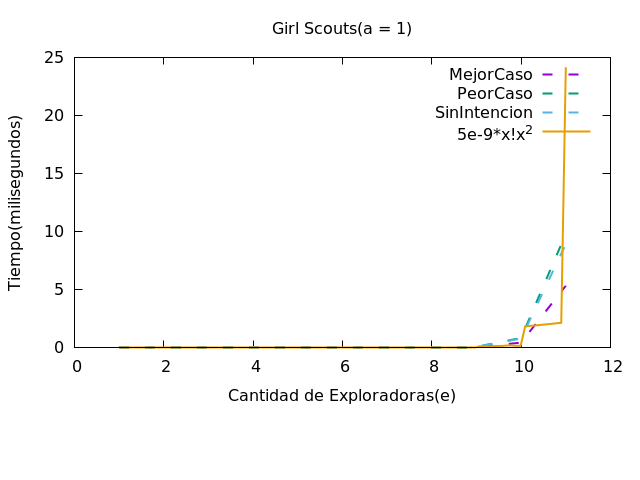
\includegraphics[width=1\textwidth]
   	 	{Imagenes/graph.png}
		\caption{Test de casos}
	\end{figure}		

\section{Apéndice:Partes relevantes del código}

\subsection{Problema 1:}
\begin{verbatim}
void calcularMaximaCantidadDeEstaciones(int kilometrosDeCable,vector<int> distanciaDeLasEstaciones){
	    
	    int inicio=0;
	    int fin=1;
	    int cantidadDeEstaciones=0;
	    int maximaCantidadDeEstaciones=0;
	    int j=0;
	    
	    while(distanciaDeLasEstaciones[j]<=kilometrosDeCable)
	    {
		         maximaCantidadDeEstaciones=j+2;
		         j++;
	    }
	    while(fin<distanciaDeLasEstaciones.size()){
	     
		         if((distanciaDeLasEstaciones[fin]-distanciaDeLasEstaciones[inicio])<=kilometrosDeCable){
			             cantidadDeEstaciones=fin-inicio+1;
			             
			             if(cantidadDeEstaciones>maximaCantidadDeEstaciones)
				                 maximaCantidadDeEstaciones=cantidadDeEstaciones;
			
			             fin++;
		         }
		         else{
			             if(fin==inicio+1){
			                	fin++;
				                 inicio++;
			             }
			             else{
				                 inicio++;
			             }
		        }
	    }
	    cout<<maximaCantidadDeEstaciones<<endl;
}
\end{verbatim}

\subsection{Probelma2:}
\begin{verbatim}
 public void agregar(int n){
	if(tamaño == 0)
		mediana = n;
	else if((tamaño % 2) == 1){ 
		if (n < mediana){ 
			menor.add(n);
			mayor.add(mediana); 
			mediana = (menor.peek() + mayor.peek()) / 2; 
		}
		else{
			mayor.add(n);
			menor.add(mediana);
			mediana = (menor.peek() + mayor.peek()) / 2;
			}
	}
	else{
		if (n < mediana){
			menor.add(n);
			mediana = menor.poll();
		}
		else{
			mayor.add(n);
			mediana = mayor.poll();
			}
	}
	tamaño++;
		
	}


\end{verbatim}

\subsection{Problema3:}
La parte de testing se encuentra en la clase FogonTest y Benchmark, donde además también hay breves comentarios describiendo el caso.
\begin{verbatim}
public void sentarExploradoras(ArrayList<Character> exploradoras, Ronda rondaAux, int tam){

if(rondaAux.size() == tam + 1 ){ 			
		    if((rondaAux.sumaDistancias(amigas) < rondaOptima.sumaDistancias(amigas)) || (rondaOptima.isEmpty()))
				rondaOptima = new Ronda(rondaAux);
				return;
		}	
		

	for(int i = 0; i < exploradoras.size(); i++){

				char e = exploradoras.get(i);
			rondaAux.add(e);
			if(rondaAux.size() == 2 && i == exploradoras.size()-1 )
			break;	
		
			if((rondaAux.sumaDistancias(amigas) >= rondaOptima.sumaDistancias(amigas)) && (rondaOptima.size() != 0 ))
				rondaAux.remove(rondaAux.size() - 1);	
			else{
				exploradoras.remove(i);
			
			sentarExploradoras(exploradoras, rondaAux,tam);
						
			char ult = rondaAux.remove(rondaAux.size() - 1);

			exploradoras.add(i,e);
			 }
		}	
		return;
	}

\end{verbatim}
\end{document}